\documentclass[a4paper]{G2-105}
\usepackage[utf8]{luainputenc}
\usepackage{listings}
\usepackage[dvipsnames]{xcolor}

\usepackage[caption=false]{subfig}

\usepackage[dvipsnames]{xcolor}
\usepackage{listings}

\graphicspath{{figures/}}

\newcommand{\CommonSoftwareRequirements}{
\begin{itemize}
\item git;
\item nvm;
\item Node.js~v6.0.0;
\item npm~v3.8.6;
\item MongoDB~v2.6.12;
\item Stardog~v4.1.
\end{itemize}
}

\newcommand{\CommonBrowserRequirements}{
\begin{itemize}
\item Google Chrome~30.0;
\item Mozilla Firefox~25.0;
\item Apple Safari~6;
\item Microsoft Internet Explorer~9.
\end{itemize}
}

\newcommand{\CommonSystemRequirements}{
\begin{itemize}
\item процессор с тактовой частотой не ниже 2.7 ГГц;
\item объем оперативной памяти не ниже 512 Мб;
\item объем жесткого диска не ниже 10 Гб.
\end{itemize}
}

\newcommand{\CommonClientRequirements}{
\begin{itemize}
\item процессор с тактовой частотой не ниже 1600 МГц;
\item объем оперативной памяти не ниже 1024 Мб;
\item объем жесткого диска не ниже 20 Гб;
\item монитор с диагональю не менее 15 дюймов;
\item манипулятор типа «мышь», клавиатура.
\end{itemize}
}

\newcommand{\CommonGoal}{повышение качества принимаемых решений по управлению отходами на предприятии за счет организации интеллектуальной поддержки процесса принятия решений на основе онтологической модели представления знаний и логического вывода на онтологии}


\newcommand{\CommonGoalCap}{Повышение качества принимаемых решений по управлению отходами на предприятии за счет организации интеллектуальной поддержки процесса принятия решений на основе онтологической модели представления знаний и логического вывода на онтологии}

\newcommand{\CommonTasks}{
\begin{itemize}
\item провести анализ процесса и специфики управления отходами на предприятии с целью построения информационно-логической модели предметной области и формирования требований к модели представления знаний;
\item разработать концепцию поддержки принятия решений по управлению отходами предприятия на основе онтологической модели представления знаний и логического вывода на онтологии;
\item разработать онтологическую модель предметной области и алгоритм генерации стратегии управления отходами предприятия на основе логического вывода на онтологии;
\item разработать и протестировать интеллектуальную систему поддержки принятия решений по управлению отходами на основе предложенных модели и алгоритма.
\end{itemize}
}

\def\CommonOntologyModelFormula{O = \left<C,~R,~F\right >}
\def\CommonOntologyModelDescription{\begin{VSTUFormulaWhereList}
\item $C$~--- конечное множество понятий (концептов) предметной области, которую представляет онтология О;
\item $R$~--- конечное множество отношений между концептами;
\item $F$~--- конечное множество функций интерпретации, заданных на концептах и/или отношениях онтологии О.
\end{VSTUFormulaWhereList}
}

\newcommand{\CommonTprFormulaCompact}{$DS = \left<S,~A,~C,~M,~P,~R\right>$, где $S$~-- описание ситуации принятия решений, состоящее из множества численных и качественных параметров: $S = \left\{P_{q1},~P_{q2},~...,~P_{qn1},~P_{qn2}\right\}$; $A$~-- множество альтернатив, каждая из которых состоит из множества управляющих воздействий: $A = \left\{A_{c1},~A_{c2},~...,\right\}$; $C$~-- множество критериев, в виде качественных оценок ситуации с точки зрения предприятия; $M$~-- модель, позволяющая для каждой альтернативы рассчитать вектор критериев; $P$~-- система предпочтений для каждого из критериев; $R$~-- решающее правило выбора альтернативы}

\def\CommonTprFormula{DS = \left<S,~A,~C,~M,~P,~R\right>}
\def\CommonTprDescription{\begin{VSTUFormulaWhereList}
\item $S$~--- описание ситуации принятия решений, состоящее из множества численных и качественных параметров, $S = \left\{P_{q1},~P_{q2},~...,~P_{qn1},~P_{qn2}~\right\}$;
\item $A$~--- множество альтернатив, каждая из которых состоит из множества управляющих воздействий: $A = \left\{A_{c1},~A_{c2},~...,~A_{cm}\right\}$;
\item $C$~--- множество критериев, в виде качественных оценок ситуации с точки зрения предприятия;
\item $M$~--- модель, позволяющая для каждой альтернативы рассчитать вектор критериев;
\item $P$~--- система предпочтений для каждого из критериев;
\item $R$~--- решающее правило выбора альтернативы.
\end{VSTUFormulaWhereList}
}

\newcommand{\CommonMetaontologyModels}{
\begin{itemize}
\item онтология отходов, описывающая их свойства и классы опасности, а также негативное влияние, которые они оказывают на окружающую среду;
\item онтология субъектов, взаимодействующих с отходами (предприятие, полигон и т. д.);
\item онтология методов управления отходами, описывающая методы (переработка, утилизации, транспортировки и т.д.) и их стоимость, экологический вред, который также должен оплачиваться субъектом согласно закону РФ.
\end{itemize}
}

\newcommand{\CommonMetaontologyFormulaCompact}{$M = \left<O_{M},~C_{M},~Inst_{M},~R_{M},~I_{M}\right>$, 

где $M$ -- метаонтологическая модель предметной области; $O_{M} = \left\{O_{W},~O_{M},~O_{S}\right\}$~-- множество онтологических моделей, объединенных в метаонтологию, $O_{W}$~-- онтология отходов, $O_{M}$~-- онтология методов управления отходами,  $O_{S}$~-- онтология субъектов управления отходами; $C_{M}$~-- конечное множество концептов, $C_{M} = \varnothing$; $Inst_{M}$~-- конечное множество экземпляров классов, $Inst_{M} = \varnothing$; $R_{M} = \left\{has,~uses,~includes\right\}$~-- конечное множество отношений метаонтологии; $I_{M}$~-- множество правил интерпретации и ограничений, $I_{M} = \varnothing$}

\def\CommonMetaontologyFormula{M = \left<O_{M},~C_{M},~Inst_{M},~R_{M},~I_{M}\right>}
\def\CommonMetaontologyDescription{\begin{VSTUFormulaWhereList}
\item $M$~--- метаонтологическая модель предметной области;
\item $O_{M}$~--- множество онтологических моделей, объединенных в метаонтологию: $O_{M} = \left\{O_{W},~O_{M},~O_{S}\right\}$, где $O_{W}$~-- онтология отходов, $O_{M}$~-- онтология методов управления отходами,  $O_{S}$~-- онтология субъектов управления отходами;
\item $C_{M}$~--- конечное множество концептов, $C_{M} = \varnothing$;
\item $Inst_{M}$~--- конечное множество экземпляров классов, $Inst_{M} = \varnothing$;
\item $R_{M}$~--- конечное множество отношений метаонтологии $M$: $R = \left\{r_{M1},~r_{M2},~r_{M3}\right\}$, где $r_{M1}$~-- отношение has «имеет», $r_{M2}$~-- отношение uses «использует», $r_{M3}$~-- отношение includes «включает»;
\item $I_{M}$~--- множество правил интерпретации и ограничений, $I_{M} = \varnothing$.
\end{VSTUFormulaWhereList}
}

\newcommand{\CommonWasteOntologyCompact}{$O_{W} = \left<C_{W},~Inst_{W},~R_{W},~I_{W}\right>$, 

где $C_{W}$~-- конечное множество концептов онтологии отходов, $C_{W} = \left\{C_{W1},~...,~C_{W26}\right\}$; $Inst_{W}$~-- множество экземпляров классов онтологии отходов, $Inst_{W} = \left\{i_{W1},~i_{W2},~...,~i_{Wj},~...,~i_{Wn}\right\}$; $R_{W}$~-- конечное множество отношений онтологии отходов: $R_{W} = \left\{r_{W1},~...,~r_{W8}\right\}$, где $r_{W1}$~-- отношение $hasHazard$, $r_{W2}$~-- отношение $hasAggregateState$, $r_{W3}$~-- relation $hasOrigin$, $r_{W4}$~-- отношение $hasAmount$, $r_{W5}$~-- отношение $hasTitle$, $r_{W6}$~-- отношение $hasEcolTax$, $r_{W7}$~-- отношение $is$, $r_{W8}$~-- отношение $is-a$; $I_{W}$~-- множество правил}

\def\CommonWasteOntologyFormula{O_{W} = \left<C_{W},~Inst_{W},~R_{W},~I_{W}\right>}
\def\CommonWasteOntologyDescription{\begin{VSTUFormulaWhereList}
\item $C_{W}$~--- конечное множество концептов онтологии отходов: $C_{W} = \left\{C_{W1},~...,~C_{W26}\right\}$;
\item $Inst_{W}$~--- множество экземпляров классов онтологии отходов: $Inst_{W} = \left\{i_{W1},~i_{W2},~...,~i_{Wj},~...,~i_{Wn}\right\}$;
\item $R_{W}$~--- конечное множество отношений онтологии отходов: $R_{W} = \left\{r_{W1},~...,~r_{W8}\right \}$, где $r_{W1}$~-- отношение $hasHazard$, $r_{W2}$~-- отношение $hasAggregateState$, $r_{W3}$~-- relation $hasOrigin$, $r_{W4}$~-- отношение $hasAmount$, $r_{W5}$~-- отношение $hasTitle$, $r_{W6}$~-- отношение $hasEcolTax$, $r_{W7}$~-- отношение $is$, $r_{W8}$~-- отношение $is-a$;
\item $I_{W}$~--- множество правил и ограничений (методика их добавления рассмотрена далее).
\end{VSTUFormulaWhereList}
}

\newcommand{\CommonMethodOntologyCompact}{$O_{M} = \left<C_{M},~Inst_{M},~R_{M},~I_{M}~\right>$, где $C_{M}$~-- конечное множество концептов онтологии методов управления отходами, $C_{M} = \left\{C_{M1},~...,~C_{M6}\right\}$; $Inst_{M}$~-- множество экземпляров классов онтологии методов управления отходами, $Inst_{M} = \left\{i_{M1},~i_{M2},~...,~i_{Mj},~...,~i_{Mn}\right\}$; $R_{M}$~-- множество отношений онтологии методов управления отходами, $R_{M} = \left\{r_{M1},~...,~r_{M8}\right\}$, где $r_{M1}$~-- отношение $is$, $r_{M2}$~-- отношение $hasTitle$, $r_{M3}$~-- отношение $hasMethod$, $r_{M4}$~-- отношение $processedBy$, $r_{M5}$~-- отношение $hasHarmfulEffect$, $r_{M6}$~-- отношение $hasCostOnDistance$, $r_{M7}$~-- отношение $hasCostOnWeight$, $r_{M8}$~-- отношение $hasCostByService$; $I_{M}$~-- множество правил интерпретации и ограничений, $I_{M} = \varnothing$}

\def\CommonMethodOntologyFormula{O_{M} = \left<C_{M},~Inst_{M},~R_{M},~I_{M}\right>}
\def\CommonMethodOntologyDescription{\begin{VSTUFormulaWhereList}
\item $C_{M}$~--- конечное множество концептов онтологии методов управления отходами: $C_{M} = \left\{C_{M1},~...,~C_{M6}\right\}$;
\item $Inst_{M}$~--- множество экземпляров классов онтологии методов управления отходами: $Inst_{M} = \left\{i_{M1},~i_{M2},~...,~i_{Mj},~...,~i_{Mn}\right\}$;
\item $R_{M}$~--- множество отношений онтологии методов управления отходами: $R_{M} = \left\{r_{M1},~...,~r_{M8}\right\}$, где $r_{M1}$~-- отношение $is$, $r_{M2}$~-- отношение $hasTitle$, $r_{M3}$~-- отношение $hasMethod$, $r_{M4}$~-- отношение $processedBy$, $r_{M5}$~-- отношение $hasHarmfulEffect$, $r_{M6}$~-- отношение $hasCostOnDistance$, $r_{M7}$~-- отношение $hasCostOnWeight$, $r_{M8}$~-- отношение $hasCostByService$;
\item $I_{M}$~--- множество правил интерпретации и ограничений, $I_{M} = \varnothing$.
\end{VSTUFormulaWhereList}
}

\newcommand{\CommonSubjectOntologyCompact}{$O_{S} = \left<C_{S},~Inst_{S},~R_{S},~I_{S}\right>$, где $C_{S}$~-- конечное множество концептов субъектов управления отходами, $C_{S} = \left\{C_{S1},~...,~C_{S6}\right\}$; $Inst_{S}$~-- множество экземпляров классов онтологии субъектов управления отходами, $Inst_{S} = \left\{i_{S1},~i_{S2},~...,~i_{Sj},~...,~i_{Sn}\right\}$; $R_{S}$~-- множество отношений онтологии субъектов управления отходами, $R_{S} = \left\{r_{S1},~...,~r_{S9}\right\}$, $r_{S1}$~-- отношение is, $r_{S2}$~-- отношение locatedIn, $r_{S3}$~-- отношение hasCoordinates, $r_{S4}$~-- отношение hasEcolOfGround, $r_{S5}$~-- отношение hasTitle, $r_{S6}$~-- отношение hasWaste, $r_{S7}$~-- отношение hasMethod, $r_{S8}$~-- отношение hasBudget, $r_{S9}$~-- отношение hasEcolOfAir; $I_{S}$~-- множество правил интерпретации и ограничений, $I_{S} = \varnothing$}

\def\CommonSubjectOntologyFormula{O_{S} = \left<C_{S},~Inst_{S},~R_{S},~I_{S}\right>}
\def\CommonSubjectOntologyDescription{\begin{VSTUFormulaWhereList}
\item $C_{S}$~--- конечное множество концептов субъектов управления отходами: $C_{S} = \left\{C_{S1},~...,~C_{S6}\right\}$;
\item $Inst_{S}$~--- множество экземпляров классов онтологии субъектов управления отходами: $Inst_{S} = \left\{i_{S1},~i_{S2},~...,~i_{Sj},~...,~i_{Sn}\right\}$;
\item $R_{S}$~--- множество отношений онтологии субъектов управления отходами: $R_{S} = \left\{r_{S1},~...,~r_{S9}\right\}$, где $r_{S1}$~-- отношение is, $r_{S2}$~-- отношение locatedIn, $r_{S3}$~-- отношение hasCoordinates, $r_{S4}$~-- отношение hasEcolOfGround, $r_{S5}$~-- отношение hasTitle, $r_{S6}$~-- отношение hasWaste, $r_{S7}$~-- отношение hasMethod, $r_{S8}$~-- отношение hasBudget, $r_{S9}$~-- отношение hasEcolOfAir;
\item $I_{S}$~--- множество правил интерпретации и ограничений, $I_{S} = \varnothing$.
\end{VSTUFormulaWhereList}
}

\def\CommonTaskGivenFormula{s = \left<Coord_{s},~L_{s},~B_{s},~W_{s},~M_{s}\right>}
\def\CommonTaskGivenDescription{\begin{VSTUFormulaWhereList}
\item $s$~--- предприятие, являющиеся экземпляром класа $Subject$ онтологии $O_{S}$;
\item $Coord_{s}$~--- координаты предприятия, строка;
\item $L_{s}$~--- локация предприятия, определяющая город, регион и др.: $L_{s} = \left\{l_{1},~l_{2},~...,~l_{i},~...,~l_{n}\right\}$, где $l_{i}$~-- экземпляр класса $Subject$ онтологии $O_{S}$;
\item $B_{s}$~--- бюджет предприятия, число;
\item $W_{s}$~--- отходы предприятия, сгрупированные по методу управления отходами $W_{s} = \left\{W_{1},~W_{2},~...,~W_{i},~...,~W_{n}\right\}$, где $W_{i}$~-- подмножество отходов, объединенных общим признаком -- метод управления $m_{i}$, $W_{i} = \left\{w_{i1},~w_{i2},~...,~w_{ij}\right\}$, где $w_{ij}$~-- экземпляр класса $Waste$ онтологии $O_{W}$;
\item $M_{s}$~--- методы управления отходами предприятия: $M_{s} = \left\{m_{1},~m_{2},~...,~m_{i},~...,~m_{n}\right\}$, где $m_{i}$~--- экземпляр класса $Method$ онтологии $O_{M}$. 
\end{VSTUFormulaWhereList}
}

\def\CommonFormalOntologyTask{M|_{min(ecol, econ)} = \{M_{1},~M_{2}~...,~M_{k}\} : k = |W_{s}|.}
\def\CommonFormalOntologySolution{St_{s} = \{\left<W_{1},~M_{1}\right>,~\left<W_{2},~M_{2}\right>,~...,~\left<W_{n},~M_{n}\right>\}.}

\newcommand{\CommonScientificNovations}{
\begin{itemize}
\item Разработана интегрированная онтологическая модель представления знаний по управлению отходами предприятия, которая отличается от известных возможностью описания данных и знаний об объектах и субъектах процесса управления отходами на общем домене концептов, а также позволяет реализовывать логический вывод на онтологии на основе семантических запросов.
\item Разработан алгоритм генерации эффективной стратегии управления отходами на основе логического вывода на онтологической модели с использованием семантических запросов.
\end{itemize}
}

\newcommand{\CommonPracticalValue}{
\begin{itemize}
\item Разработанные в диссертационной работе модели и алгоритм позволяют производить генерацию эффективной стратегии управления отходами на предприятии. Реализованная система поддержки принятия решений включает в себя модуль генерации стратегии управления отходами на предприятии, а также онтологическую базу знаний отходов, методов и субъектов управления отходами. Разработана методика создания и расширения онтологической базы знаний предметной области, что позволяет применять данную систему, учитывая особенности различных субъектов управления отходами и видов отходов. В результате повышается качество принимаемых решений в области обращения с отходами на предприятии при использовании предложенной системой стратегии управления отходами.
\item Реализованная система поддержки принятия решений прошла аппробацию в учреждении ГБУЗ «Николаевское ЦРБ» в процессе обращения с отходами. 
\item Работа выполнена при поддержке РФФИ в рамках проекта №15-07-03541 «Интеллектуальная поддержка принятия решений по управлению сложными системами на основе интеграции различных типов рассуждений на знаниях, представленных онтологической моделью».
\end{itemize}
}

\newcommand{\CommonResults}{
\begin{itemize}
\item Проведен анализ процессов управления отходами на предприятии; информационных систем, используемых при принятии решений по управлению отходами; обзор моделей и методов, используемых при поддержке принятия решений по управлению отходами. Основным недостатком существующего процесса является сложность и трудоемкость процесса принятия верного решения экпертом в области управления отходами на предприятии. Построена информационно-логическая модель предметной области, включающая функциональную и объектную модели. Выявлены требования к модели представления знаний для описания объектов и субъектов процесса управления отходами на предприятии.
\item Разработана концепция поиска эффективной стратегии управления отходами на предприятии. Предложенная концепция предполагает создание автоматизированной системы для решения задачи генерации стратегии управления отходами, что позволяет сократить трудоемкость решения задачи и повысить обоснованность принимаемых решений, за счет применения моделей и методов искусственного интеллекта -- онтологической модели представления знаний и логического вывода на онтологиях.
\item Разработана интегрированная онтологическая модель представления знаний предметной области, состоящая из следующих компонентов, объединенных метаонтологией: (1) онтология отходов; (2) онтология методов управления отходами; (3) онтология субъектов управления отходами. Разработанная модель позволяет описывать объекты и субъекты процесса управления отходами на общем домене концептов и решать задачу поиска эффективной стратегии управления отходами посредством логического вывода на онтологии. Разработан алгоритм генерации эффективной стратегии управления отходами на предприятии на основе логического вывода на онтологической модели с использованием языка семантических запросов.
\item Разработана архитектура и реализована интеллектуальная система поддержки принятия решений для генерации эффективной стратегии управления отходами на предприятии на основе описанных моделей и алгоритма. Проведено тестирование системы и проверка соответствия полученой стратегии управления отходами с данными по учреждению ГБУЗ «Николаевское ЦРБ». Стратегия управления отходами, полученная в результате генерации системой, соответствует сформулированным критериям эффективности и соответствует выбранным методом управления отходами, примененным учреждением ГБУЗ «Николаевское ЦРБ». Данный результат позволяет сделать вывод об эффективности разработанных моделей и алгоритма.
\end{itemize}
}

\newcommand{\CommonKeywords}{Ключевые слова: управление отходами, поддержка принятия решений, метаонтология, OWL-DL, логический вывод на онтологии, RDF, SPARQL, интеллектуальная система поддержки принятия решений}
\newcommand{\CommonKeywordsEng}{Keywords: waste management, decision support, Metaontology, OWL-DL, inference logical consequences, RDF, SPARQL, Intelligent Decision Support System}

\newcommand{\CommonPublicationsVAK}{
\begin{enumerate}
\item Кульцова,~М.Б. Интеллектуальная поддержка принятия решений по управлению отходами на городских территориях на основе онтологической модели представления знаний~/ Кульцова~М.Б., Руднев~Р.Ю., Жукова~И.Г., Аникин~А.В.~//~Изв. ВолгГТУ. Серия «Актуальные проблемы управления, вычислительной техники и информатики в технических системах». Вып. 13~:~межвуз. сб. науч. ст.~/~ВолгГТУ.~--~Волгоград,~2015.~--~№ 13 (117).~-- C.~104-109.
\end{enumerate}
}

\newcommand{\CommonPublicationsOther}{
\begin{enumerate}
\setcounter{enumi}{1}

\item Руднев,~Р.Ю. Онтологический подход к поддержке принятия решений по управлению отходами на городских территориях~/~Руднев~Р.Ю., Кульцова~М.Б., Жукова~И.Г.~//~XII Международная научно-практическая конференция «Инновации на основе информационных и коммуникационных технологий» ИНФО-2015 (Сочи, 1-10 окт. 2015 г.)~:~сб. науч. ст.~--~Сочи, 2015.~--~С.~568-571.

\item Руднев,~Р.Ю. Концепция поддержки принятия решений по управлению отходами на городских территориях на основе онтологического и имитационного моделирования~/~Руднев~Р.Ю., Кульцова~М.Б.~//~XX региональная конференция молодых исследователей Волгоградской области (Волгоград, 10-13 нояб. 2015 г.)~:~тез. докл.~/~отв. ред. А.В. Навроцкий~;~Волгогр. гос. техн. ун-т [и др.].~--~Волгоград, 2016.~--~C.~143-144.

\item Kultsova~M. An ontology-based approach to intelligent support of decision making in waste management~/~Kultsova~M., Rudnev~R., Anikin~A., Zhukova~I.~//~CIT DS Creativity in Intelligent Technologies Data Science, The 7th International Conference on Information, Intelligence, Systems and Applications,~IISA2016,~Greece,~2016 (принята к публикации).

\end{enumerate}
}

\newcommand{\CommonPublications}{
\begin{enumerate}

\item [1] Кульцова,~М.Б. Интеллектуальная поддержка принятия решений по управлению отходами на городских территориях на основе онтологической модели представления знаний~/ Кульцова~М.Б., Руднев~Р.Ю., Жукова~И.Г., Аникин~А.В.~//~Изв. ВолгГТУ. Серия «Актуальные проблемы управления, вычислительной техники и информатики в технических системах». Вып. 13~:~межвуз. сб. науч. ст.~/~ВолгГТУ.~--~Волгоград,~2015.~--~№ 13 (117).~-- C.~104-109.

\item [2] Руднев,~Р.Ю. Онтологический подход к поддержке принятия решений по управлению отходами на городских территориях~/~Руднев~Р.Ю., Кульцова~М.Б., Жукова~И.Г.~//~XII Международная научно-практическая конференция «Инновации на основе информационных и коммуникационных технологий» ИНФО-2015 (Сочи, 1-10 окт. 2015 г.)~:~сб. науч. ст.~--~Сочи, 2015.~--~С.~568-571.

\item [3] Руднев,~Р.Ю. Концепция поддержки принятия решений по управлению отходами на городских территориях на основе онтологического и имитационного моделирования~/~Руднев~Р.Ю., Кульцова~М.Б.~//~XX региональная конференция молодых исследователей Волгоградской области (Волгоград, 10-13 нояб. 2015 г.)~:~тез. докл.~/~отв. ред. А.В. Навроцкий~;~Волгогр. гос. техн. ун-т [и др.].~--~Волгоград, 2016.~--~C.~143-144.

\item [4] Kultsova~M. An ontology-based approach to intelligent support of decision making in waste management~/~Kultsova~M., Rudnev~R., Anikin~A., Zhukova~I.~//~CIT DS Creativity in Intelligent Technologies Data Science, The 7th International Conference on Information, Intelligence, Systems and Applications,~IISA2016,~Greece,~2016.

\end{enumerate}
}

% Информация для генерации титульных листов, хедеров и футеров
\VSTUSetDocumentNumbersPrefix{}
\VSTUSetDocumentCode{МД-40-461-806-10.19-09.04.04-08-16}
\VSTUSetDocumentTypeDative{магистерской диссертации}
\VSTUSetDocumentTypeAccusative{магистерскую диссертацию}
\VSTUSetDocumentTypeEng{master's thesis}
\VSTUSetInitialData{задание, выданное научным руководителем кафедры ПОАС, утвержденное приказом ректора университета}
\VSTUSetOrder{1551--ст}{20}{октябрь}{2014}
\VSTUSetDeadline{01}{июня}
\VSTUSetFaculty{Электроники и вычислительной техники}
\VSTUSetDepartment{Программное обеспечение автоматизированных систем}
\VSTUSetDepartmentCode{10.19}
\VSTUSetDirection{09.04.04 Программная инженерия}
\VSTUSetHeadOfDepartment{Зав. кафедрой ПОАС}{д.т.н., проф.}{А. М. Дворянкин}{Дворянкин Александр Михайлович}
\VSTUSetDirector{доц. каф. ПОАС}{к.т.н.}{М. Б. Кульцова}{Кульцова Марина Борисовна}
\VSTUSetStandardsAdviser{ст. преп. каф. ПОАС}{}{О. Н. Ляпина}{Ляпина Ольга Николаевна}
\VSTUSetReviewer{доц. каф. САПР и ПК}{д.т.н., проф.}{Н. П. Садовникова}{Садовникова Наталья Петровна}
\VSTUSetStudent{ПРИН-2Н}{Р. Ю. Руднев}{Руднев Роман Юрьевич}{Руднева Романа Юрьевича}
\VSTUSetStudentFullNameEng{Roman Rudnev}
\VSTUSetTitle{Интеллектуальная система поддержки принятия  решений  по  управлению  отходами}
\VSTUSetTitleEng{Intelligent decision support system of waste management}

% Определние цветов
\definecolor{dimgray}{HTML}{696969}
\definecolor{silver}{HTML}{C0C0C0}
\definecolor{darkgray}{HTML}{A9A9A9}

% Определение стилей
\lstdefinestyle{appendix}{
xleftmargin=8mm,
captionpos=b,
basicstyle=\ttfamily\footnotesize,
breakatwhitespace=false, 
breaklines=true,
keepspaces=true,
showspaces=false,
showstringspaces=false,
showtabs=false,                  
tabsize=2,
frame=single,
numbers=left,
stepnumber=1,
numbersep=7pt,
numberstyle=\footnotesize\color{silver}
}

\lstdefinestyle{default}{
basicstyle=\ttfamily\small,
xleftmargin=8mm,
breakatwhitespace=false,         
breaklines=true,                 
captionpos=b,                    
keepspaces=true,
showspaces=false,                
showstringspaces=false,
showtabs=false,                  
tabsize=2,
}

% Определение поддержки формата Turtle
\lstdefinelanguage{ttl}{
sensitive=true,
morecomment=[l][\color{dimgray}]{@},
morecomment=[l][\itshape\color{darkgray}]{\#},
morestring=[b]",
morekeywords={rdf,rdfs,owl,xsd}
}


\makeatletter
\def\verbatim@font{\normalfont\rmfamily}
\preto{\@verbatim}{\topsep=0pt \partopsep=0pt }
\makeatother

\lstset{style=default}

\graphicspath{{figures/}}

\begin{document}


%
\VSTUInitializeAvtoreferat
%

\thispagestyle{empty}

Работа выполнена на кафедре «Программное обеспечение автоматизированных систем» Волгоградского Государственного Технического Университета.

Научный руководитель: \VSTUDirectorDegreeAndPost{} \VSTUDirectorFullName{}

%Ведущая организация: Волгоградский Государственный Технический университет

%Защита состоится на заседании диссертационного совета при Волгоградском государственном 
%техническом университете по адресу 400005, Россия, Волгоград, пр. Ленина 28.

\vfill

%Ученый секретарь диссертационного совета

\newpage

\starchapter{ОБЩАЯ ХАРАКТЕРИСТИКА РАБОТЫ}

\textbf{Актуальность темы исследования}.
В статье Федерального закона РФ от 24.06.1998 № 89-ФЗ «Об отходах производства и потребления» сказано, что отходы производства и потребления — это остатки материалов, сырья, иных изделий или продуктов, которые образовались в процессе потребления или производства, а также продукция или товары, которые утратили свои потребительские свойства. Следовательно, любая организация в процессе своей деятельности (не только производящая отходы, но также потребляющая товары и отходы) образует отходы, которые должны быть учтены. После образования отходов они должны быть направлены на обезвреживание, переработку или захоронение (в зависимости от вида отхода) в соответствии с законами, правилами и нормами. В частности, утилизация отходов и вывоз мусора должны осуществляться лицензированными предприятиями. В случае несоблюдения экологических требований при обращении с отходами в соответствии со статьей 8.2 Кодекса РФ об административных правонарушениях подобные нарушения влекут за собой наложение административного штрафа.

Большое число связанных задач управления отходами и их высокая сложность требуют системного подхода в вопросах управления отходами и применения современных информационных технологий. Под системой управления отходами понимают совокупность взаимосвязанных мероприятий по переработке, сбору, хранению и использованию отходов, а также контролем за данными процессами. Эффективная система управления отходами должна строиться не только на соответствующих нормативно-правовых актах, традиционных технологиях и методах минимизации отходов, но также учитывать региональную специфику экологических проблем, применять экономические механизмы, использовать современные инновационные технологии управления. К таким технологиям относятся различные специализированные программно-информационные системы в сфере обращения с отходами (системы документооборота, геоинформационные системы, системы поддержки принятия решений и др.), в которых используются различные подходы к поддержке принятия решения по управлению отходами, в том числе и интеллектуальные. Однако необходим комплексный подход, который не только позволял бы находить выгодные с экономической точки зрения стратегии управления отходами на предприятии, но также учитывал особенности законодательства РФ в сфере обращения с отходами, в том числе и для каждого конкретного региона. При этом должна иметься возможность расширения и усовершенствования системы по мере изменения подходов к управлению и методик переработки отходов, а также субъектов обращения с отходами. 

\textbf{Целью работы} является \CommonGoal.

Для достижения поставленной цели были поставлены и выполнены следующие задачи:
\CommonTasks

\textbf{Объектом исследования} в диссертационной работе является процесс управления отходами на предприятии.

\textbf{Предметом исследования} является интеллектуальная поддержка принятия решений по управлению отходами.

\textbf{Методы исследований}. Для решения поставленных задач были использованы методы искусственного интеллекта, системного анализа, семантические технологии (Semantic Web) -- методы метаописаний на основе онтологий, методы логического вывода на онтологиях на основе семантических запросов.

\textbf{Научная новизна работы} заключается в следующем:
\CommonScientificNovations

\textbf{Практическая ценность работы} заключается в следующем:
\CommonPracticalValue

\textbf{Положения, выносимые на защиту}:
\begin{itemize}
\item интегрированная онтологическая модель представления знаний, включающая следующие компоненты: метаонтологию предметной области управления отходами, онтологию отходов, онтологию методов управления отходами, онтологию субъектов управления отходами;
\item алгоритм генерации эффективной стратегии управления отходами на предприятии на основе
логического вывода на онтологиях с использованием языка семантических запросов;
\item архитектура и реализация интеллектуальной системы поддержки принятия решений по управлению отходами на основе разработанных моделей и алгоритмов.
\end{itemize}

\textbf{Апробация работы}. Основные положения и материалы диссертации докладывались
на международной научно-практической конференции «Инновации на основе информационных и коммуникационных технологий» (ИНФО-2015); отборе в программу во всероссийский инновационный конкурс «УМНИК» по Волгоградской области, Волгоград 2015; XX региональной конференции молодых исследователей Волгоградской области, Волгоград 2015.

\textbf{Публикации}. По теме диссертации были опубликованы 4 научные статьи, в том числе одна из них в журнале из списка ВАК.

\starchapter{СОДЕРЖАНИЕ РАБОТЫ}

В \textbf{первой главе} проведен анализ современного состояния вопроса, сформулированы цель и задачи исследования. Проведен обзор существующих моделей и методов поддержки принятия решений по управлению отходами и их реализации в системах поддержки принятия решений.

В настоящее время на федеральном уровне действует большое количество нормативных правовых актов, регулирующих обращение с отходами производства и потребления, центральное место среди которых занимают федеральный закон «Об охране окружающей среды» и «Об отходах производства и потребления». В нем определяется термин управление отходами  (или обращение с отходами) -- это деятельность, в процессе которой образуются отходы, а также деятельность по сбору, использованию, обезвреживанию, транспортированию и размещению отходов.

Система управления отходами РФ состоит из процесса разработки и принятия необходимой нормативно-правовой базы на всех уровнях государства, начиная с федерального уровня, а также производственной деятельности, учета и контроля со стороны государственных структур.

В процессе обращения с отходами предприятие испытывает целый ряд проблем различного содержания. К ним относятся: отсутствие полной информации о постоянно растущих объемах образованных отходов, увеличение затрат на транспортировку, размещение и утилизацию отходов, связанную с ежегодным увеличением стоимости услуг, недостатком актуальных сведений о расположении перерабатывающих предприятий и полигонов отходов, количестве и видах хранимых там отходах, информации о незаконных свалках и экологических зонах где они располагаются. Все эти обозначенные трудности осложняют процесс принятия решений по управлению отходами. Для того, чтобы облегчить процесс принятия решения по управлению отходами, создаются специализированные автоматизированные инструменты, которые можно подразделить на следующие группы: системы документооборота (программные комплексы «Русь», «Региональный кадастр отходов», «Отходы-регион», «Око»), геоинформационные системы («Юнидо», «Чистый город») и системы поддержки принятия решений (LCA-IWM, SMART, SCOLDSS). Однако необходим подход, позволяющий учитывать специфику законов РФ в области обращения с отходами и помогать лицу, принимающему решения, предлагая возможные стратегии управления отходами на предприятии.

В настоящей работе рассматривается только процесс поддержки принятия решений по управлению отходами на предприятии. Для поддержки принятия решений c помощью информационных технологий, включая анализ и выработку альтернатив, в системах в основном используются следующие модели и методы: информационный поиск, интеллектуальный анализ данных, извлечение знаний из баз данных, рассуждения на основе прецедентов, рассуждения на правилах, искусственные нейронные сети, генетические алгоритмы, имитационное моделирование, качественное моделирование, нечеткое моделирование.

Таким образом, актуальна проблема автоматизации поддержки принятия решений по управлению отходами на предприятии. Для решения данной проблемы представляется перспективным использование онтологических моделей для описания предметной области управления отходами. Использование онтологий позволит с помощью реализации логического вывода генерировать возможную стратегию управления отходами. Поэтому необходимо разработать онтологическую модель описания субъектов и объектов процесса обращения с отходами, алгоритм генерации эффективной стратегии управления отходами на предприятии на основе логического вывода на онтологии и реализовать автоматизированную систему поддержки принятия решений.

Во \textbf{второй главе} в результате проведенного обзора законов, регламентирующих процесс обращения с отходами, и анализа системы управления отходами РФ, представлен многоуровневый процесс формирования системы управления отходами на предприятии (см. рисунок~\ref{fig:as_is}).

На первом уровне (организационном, административном) предприятие ориентируется на исполнение требований, предъявляемых законодательством РФ в области обращения с отходами.
На втором уровне (консультативно-аналитическом) производится аудит отходов и анализ проектных документов для выявления приоритетных направлений в области обращения с отходами, требующих улучшения. Вырабатывается стратегия обращения с отходами: минимизация их образования, вторичное использование отходов, сокращение использования сырья, утилизация образованных отходов или их экологически безопасное размещение. На третьем уровне (уровне внедрения) осуществляется принятие управленческих решений о внедрении отобранных технологий минимизации отходов, энерго- и ресурсосберегающих технологий, технологий переработки отходов и т.д. На последнем уровне процесса систематизируется опыт, накопленный на предыдущих уровнях в результате использования административных и аналитических инструментов, применения новых технологических и технических решений, управленческого консультирования. Итогом процесса формирования является система управления отходами на предприятии.

\begin{figure}[H]
\centering
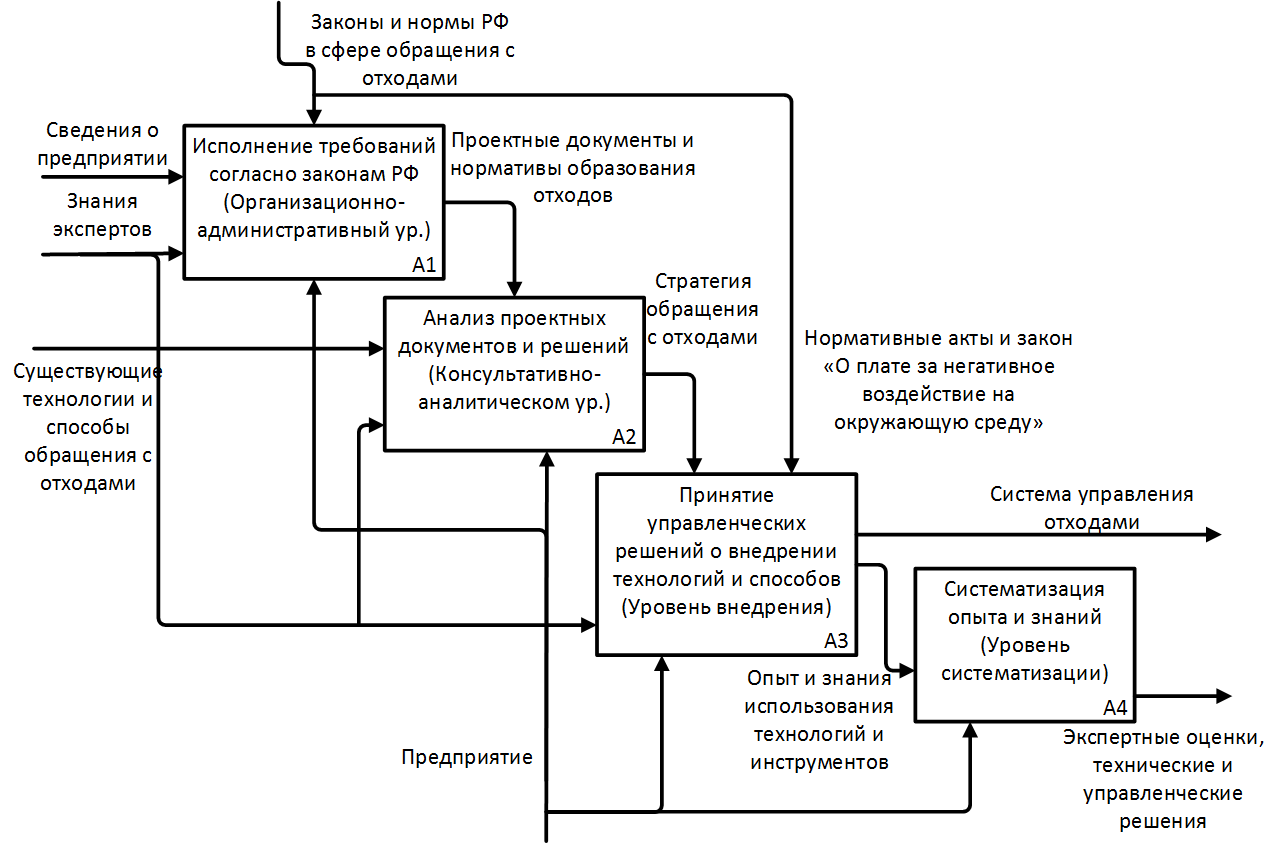
\includegraphics[scale=0.6]{as_is}
\caption{Диаграмма IDEF0. Процесс формирования системы управления отходами на предприятии}
\label{fig:as_is}
\end{figure}

Далее сформулирована задача принятия решений по управлению отходами на предприятии: \CommonTprFormulaCompact. Данная задача решается лицом, принимающим решение (ЛПР), с привлечением в качестве консультантов экспертов по смежным предметным областям (например, экологов).

В процессе проведения исследования для построения объектной модели предметной области управления отходами были выявлены объекты и субъекты процесса обращения с отходами, их характеристики и отношения между ними (см. рисунок~\ref{fig:er}). Подробное описание объектной модели предметной области приведено в диссертации.

\begin{figure}[H]
\centering
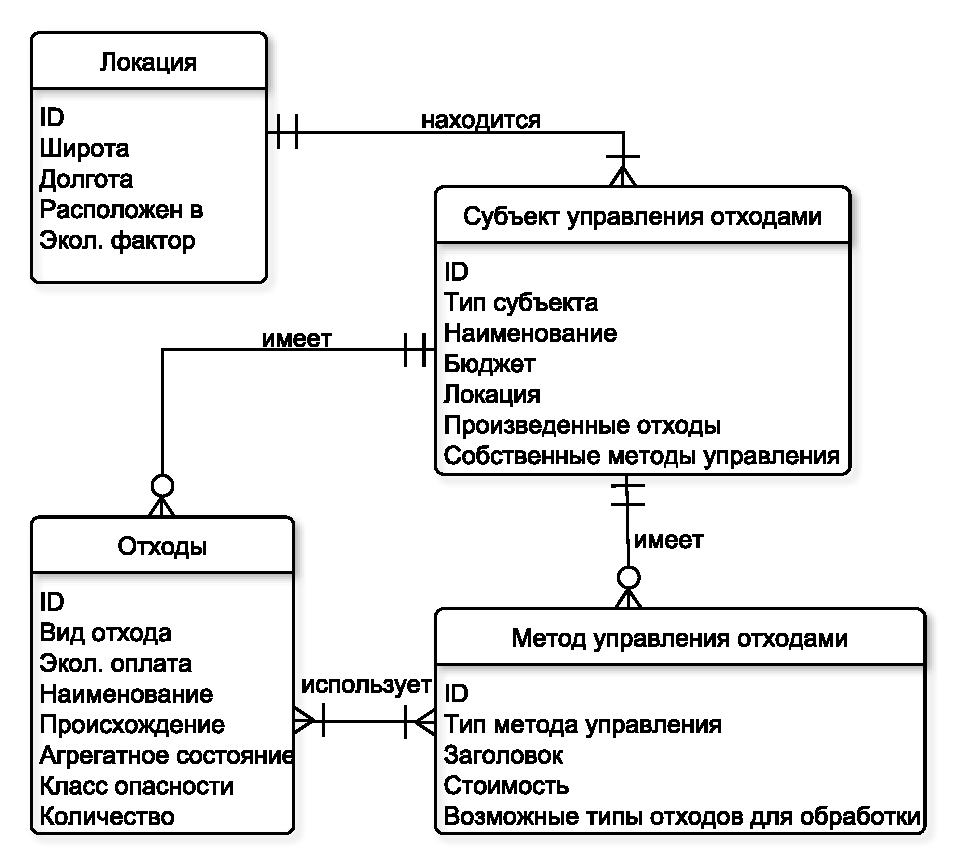
\includegraphics[scale=0.6]{er}
\caption{ER-диаграмма предметной области управления отходами}
\label{fig:er}
\end{figure}

На основании результатов исследования сформулированы требования к модели представления знаний и данных. Для представления знаний выбрана онтологическая модель. Онтология сочетает в себе достоинства ряда других моделей представления знаний, позволяет описывать структуру объектов предметной области и интегрировать рассматриваемые модели на основе общих компонент, поддерживает описание и доступ к знаниям в открытых средах. В качестве языка описания онтологий выбран язык OWL DL, рекомендованный консорциумом W3C и поддерживаемый множеством инструментальных средств.

В заключение предложена концепция поиска эффективной стратегии управления отходами на предприятии на основе онтологической базы знаний и логического вывода на онтологии с использованием семантических запросов (см. рисункок~\ref{fig:wm_concept}). Под стратегией управления отходами понимается комплекс методов управления для каждой группы отходов предприятия. При этом эффективной считается такая стратегия, в которой выбранные методы управления отходами обладают наименьшей экономической стоимостью, а также полностью соответствуют законам и нормам РФ.

\begin{figure}[H]
\centering
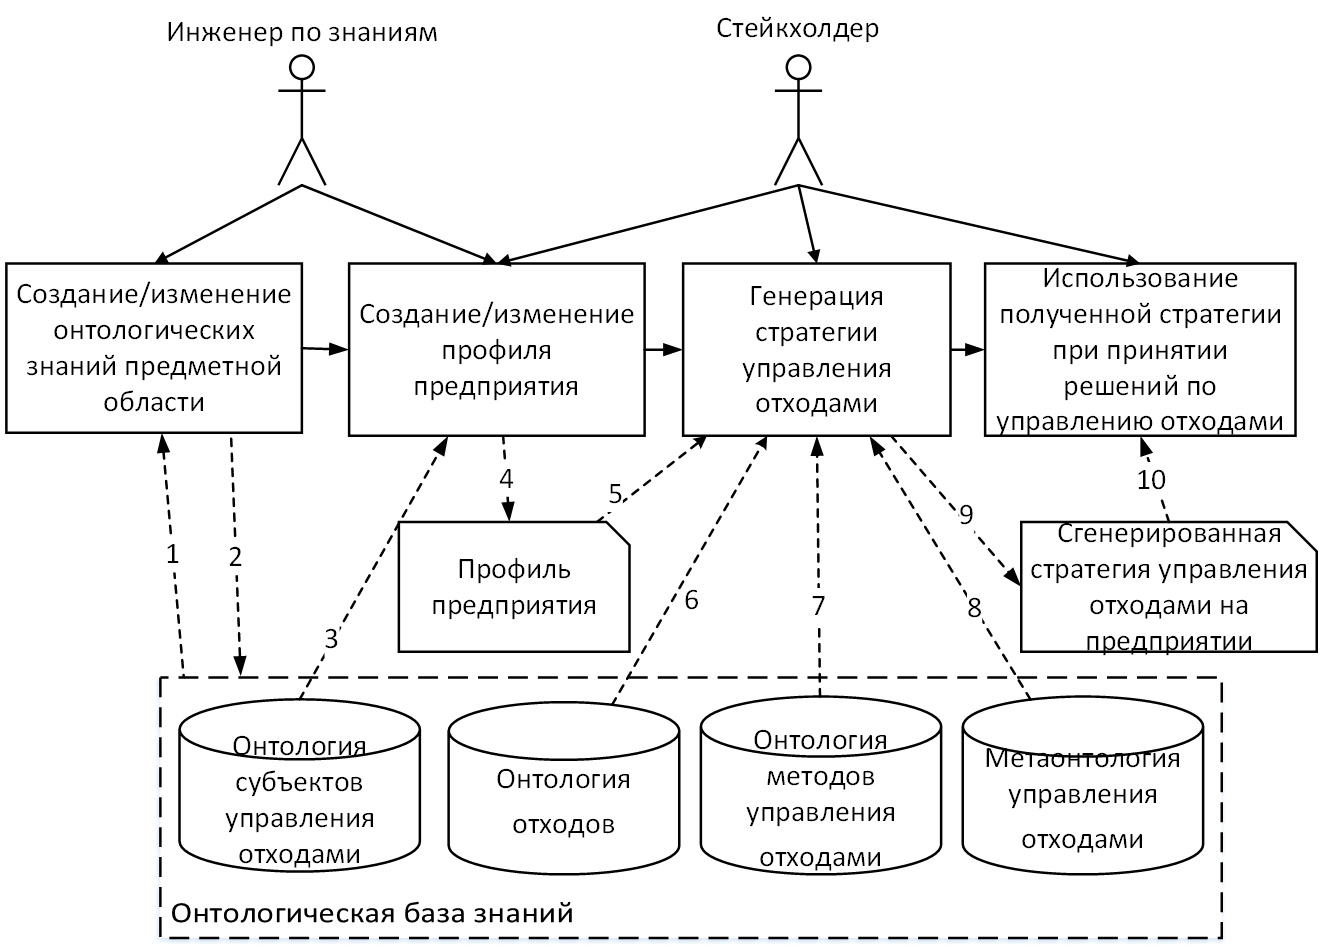
\includegraphics[scale=0.5]{wm_concept}
\caption{Концепция поиска эффективной стратегии управления отходами предприятия с использованием онтологий}
\label{fig:wm_concept}
\end{figure}

Процесс генерации эффективной стратегии управления отходами состоит из следующих этапов:
\begin{itemize}
\item [1] Cоздать новую (1) или изменить существующую онтологическую базу знаний (2) управления отходами, включающую онтологию отходов, онтологию методов управления и онтологию субъектов управления отходами.
\item [2] На основе разработанной онтологии субъектов управления отходами (3) задать профиль предприятия (4). 
Профиль предприятия описывает бюджет, географическое положение, отходы предприятия, собственные способы обращения с ними и др.
\item [3] На основе профиля предприятия (5), онтологии отходов (6), онтологии методов управления с отходами (7) и метаонтологии в целом (8) сгенерировать стратегию управления отходами на предприятии (9).
\item [4] Использовать полученную стратегию при принятии решений по управлению отходами (10).
\end{itemize}

Этапы 1-4 выполняются либо с помощью графического интерфейса разработанной системы, либо с помощью редактора онтологий согласно методике создания и расширения базы знаний. Этапы 5-9 выполняются системой с использованием логического вывода на онтологиях и семантических запросов.

В \textbf{третьей главе} на основе проведенного анализа предметной области, выявленных требований к модели представления знаний и предложенной концепции поиска стратегии управления отходами, разработана интегрированная онтологическая модель представления знаний.

Для интеграции компонентов описания объектов и субъектов предметной области управления отходами и отношений между ними, разработана метаонтология (см. рисунок~\ref{fig:metaontology}).

Метаонтология включает в себя следующие онтологии: \CommonMetaontologyModels

Формальная модель метаонтологии имеет следующий вид:

\CommonMetaontologyFormulaCompact.

\begin{figure}[H]
\centering
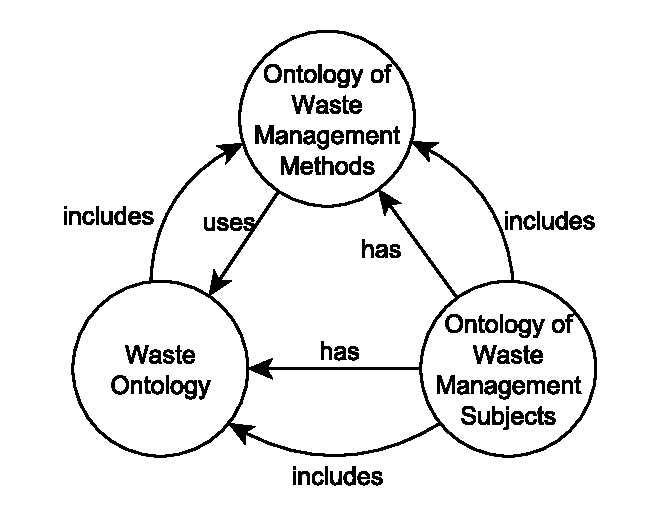
\includegraphics[scale=0.8]{metaontology}
\caption{Диаграмма IDEF5 метаонтологической модели управления отходами}
\label{fig:metaontology}
\end{figure}

Онтология отходов (см. рисунок~\ref{fig:waste_ontology}) имеет вид: 

\CommonWasteOntologyCompact. 

Онтология описывает отходы, классифицируя их по классу опасности, агрегатному состоянию, происхождению и методу управления. В последующем такое описание онтологии может быть расширено новыми видами отходов путем добавления новых классов-наследников.

Всего онтология отходов  включает описание 23 видов отходов на основе множества семантических правил.

\begin{figure}[H]
\centering
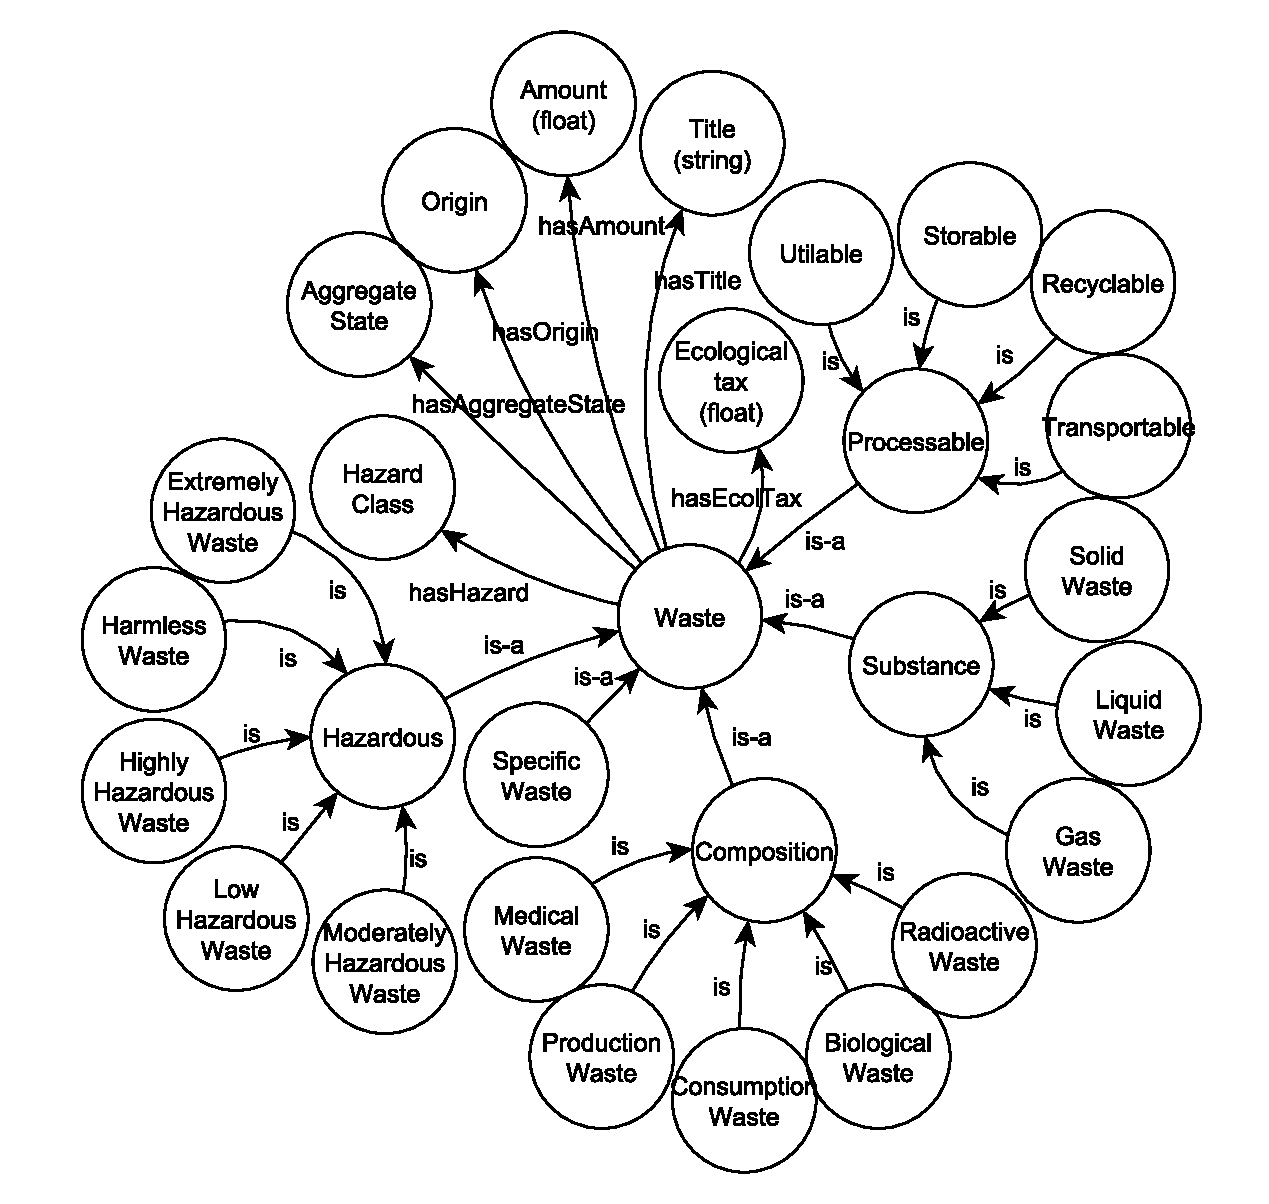
\includegraphics[scale=0.6]{waste_ontology}
\caption{Диаграмма IDEF5 онтологии отходов}
\label{fig:waste_ontology}
\end{figure}

Пример такого определения вида отхода с использованием семантических правил в формате Turtle имеет следующий вид:
\begin{verbatim}
:W23 a owl:Class;
     rdfs:subClassOf :SpecificWaste,
     [a owl:Restriction;
       owl:onProperty :hasMethod;
       owl:someValuesFrom :Recycling],
     [a owl:Restriction;
       owl:onProperty :hasMethod;
       owl:someValuesFrom :Transportation],
     [a owl:Restriction;
       owl:onProperty :hasMethod;
       owl:someValuesFrom :Utilization],
     [a owl:Restriction;
       owl:onProperty :hasAggregateState;
       owl:hasValue :solid],
     [a owl:Restriction;
       owl:onProperty :hasHazardClass;
       owl:hasValue :fiveClass],
     [a owl:Restriction;
       owl:onProperty :hasOrigin;
       owl:hasValue :consumption];
     [a owl:Restriction;
       owl:onProperty :hasOrigin;
       owl:hasValue :consumption];
     rdfs:label «Отходы бумаги и картона от канцелярской деятельности»@ru.
\end{verbatim}

Данное правило можно интерпретировать следующим образом: отходы бумаги и картона от канцелярской деятельности являются твердыми, имеют бытовое и промышленное происхождение, обладают пятым классом опасности, и к ним могут быть применены методы утилизации, переработки и транспортировки.

Остальные онтологии являются таксономиями (не включают в себя DL-правил) и подробно описаны в диссертации. Онтология субъектов управления отходами описывает 12 предприятий. Всего  разработанная в рамках работы онтология включает в себя 794 аксиомы (axiom), из которых 566 являются логическими аксиомами (logical axiom), а также: 62 класса (class), 8 объектных свойств (object property), 9 свойств данных (data property) и 82 экземпляра классов (individual).

На разработанной онтологической модели поставлена задача генерации эффективной стратегии управления отходами предприятия. Пусть задан профиль некоторого предприятия: 

$s = \left<Coord_{s},~L_{s},~B_{s},~W_{s},~M_{s}\right>$, 

где $s$~--- предприятие, являющиеся экземпляром класа $Company$ онтологии $O_{S}$; $Coord_{s}$~--- координаты предприятия, строка; $L_{s}$~--- локация предприятия, определяющая город, регион и др.: $L_{s} = \left\{l_{1},~l_{2},~...,~l_{i},~...~\right\}$, где $l_{i}$~--- экземпляр класса $Subject$ онтологии $O_{S}$; $B_{s}$~--- бюджет предприятия, число; $W_{s}$~--- отходы предприятия, $W_{s} = \left\{w_{1},~w_{2},~...,~w_{i},~...~\right\}$, где $w_{i}$~--- экземпляр класса $Waste$ онтологии $O_{W}$; $M_{s}$~--- способы управления отходами предприятия: $M_{s} = \left\{m_{1},~m_{2},~...,~m_{i},~...~\right\}$, где $m_{i}$~--- экземпляр класса $Method$ онтологии $O_{M}$. Необходимо:
\begin{enumerate}
\item [1] На основании возможных по закону РФ методов управления отходами, разбить множество отходов $W_{s}$ на подмножества $W_{M_{i}}$ (см. рисунок~\ref{fig:task_group_method}), так что $W_{M_{i}} = \left\{w_{1},~w_{2},~...~\right\}$, где  $M_{i}$~--- способ управления отходами; $M_{i}=\left\{m_{1},~m_{2},~...,~m_{j},~...~\right\}$, где $m_{j}$~--- экземпляр класса $Method$ онтологии $O_{M}$.
\item [2] Найти методы управления отходами, обладающие минимальной стоимостью, то есть экономической стоимостью услуги и суммой экологического платежа. (см. рисунок~\ref{fig:task_best_method}), то есть $C = \sum w_{j} \cdot c_{i} \rightarrow min$, где $c_{j}$~--- стоимость применения метода $m_{j} \in M_{i}$ : $i=1,~...,~n$; $j=1,~...,~|W_{M_{i}}|$.
\item [3] Сформировать эффективную стратегию управления отходами предприятия: $St_{s} = \{\left<W_{M_{1}},~M_{1}\right>,~...,~\left<W_{M_{i}},~M_{i}\right>,~...,~\left<W_{M_{n}},~M_{n}\right>\}$, где $M_{i}=\left\{m_{1},~m_{2},~...~\right\}$.
\end{enumerate}

\begin{figure}
\centering
\renewcommand{\thesubfigure}{а}
\subfloat[1][Группировка отходов по методам управления]{
  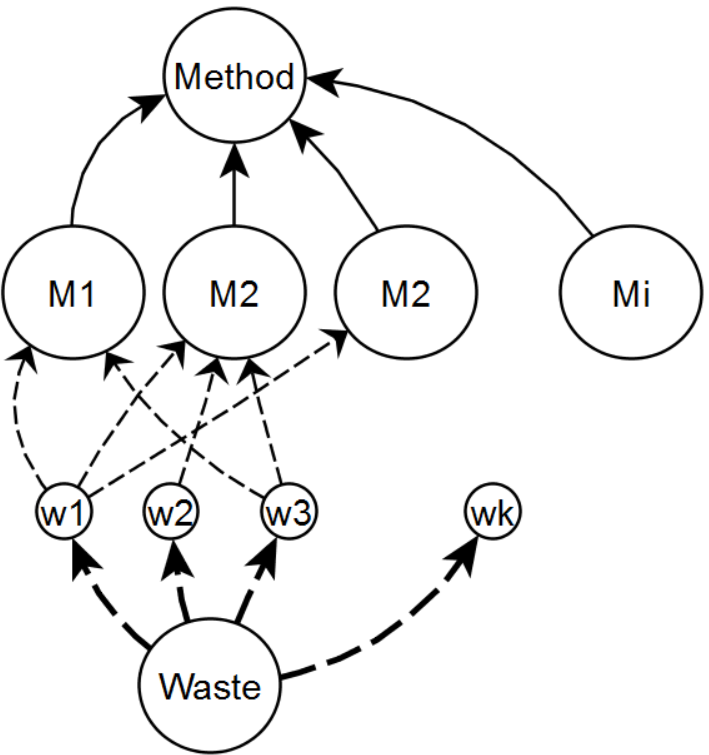
\includegraphics[scale=0.54]{task_group_method}
  \label{fig:task_group_method}
}
\renewcommand{\thesubfigure}{б}
\subfloat[Поиск минимальных по стоимости методов управления]{
  \centering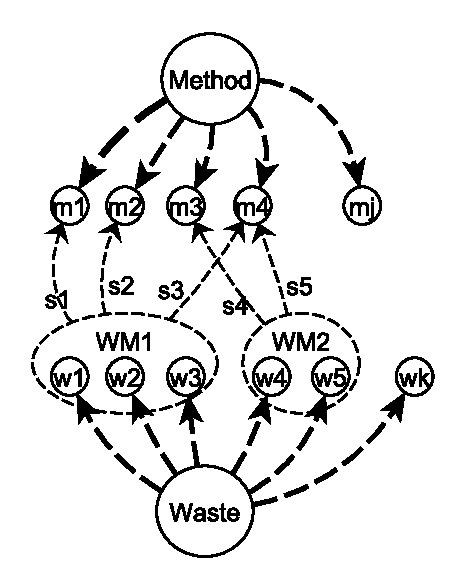
\includegraphics[scale=0.54]{task_best_method}
  \label{fig:task_best_method}
}
\caption{Схема поиска стратегии управления отходами}
\label{fig:main}
\end{figure}

Далее в диссертации описана методика создания и расширения онтологической базы знаний управления отходами и представлен пример ее применения на основе сведений об учреждении ГБУЗ «Николаевское ЦРБ».

Алгоритм генерации эффективной стратегии управления отходами на предприятии с использованием логического вывода на онтологиях и семантических запросов представлен на рисунке~\ref{fig:algorithm}. Для реализации 1, 2 и 3 шага алгоритма разработаны семантические запросы на языке SPARQL. В частности, для получения возможных методов управления отходами используется следующий шаблон SPARQL-запроса:
\begin{verbatim}
select distinct ?type ?title ?waste
where {
    ?waste a ?wasteType.
    ?wasteType rdfs:subClassOf :SpecificWaste,
       [a owl:Restriction;
         owl:onProperty :hasMethod;
         owl:someValuesFrom ?type].
    ?type rdfs:label ?title.
    filter(?waste in (:id1, :id2, ..., :idn))
}
\end{verbatim}

В данном шаблоне ?title, ?type, ?waste, ?wasteType -- это обозначение переменных SPARQL-запроса: ?title -- наименование способа управления отходами, ?type -- тип метода управления отходами, ?waste -- конкретный отход для которго происходит выборка (:id1,~...~:idn~-- экземпляры класса :SpecificWaste), ?wasteType -- вид отхода.

Аналогично определены семантические запросы для получения данных о предприятии, его отходах и возможных методах управления отходами.

Таким образом, разработанный алгоритм позволяет генерировать эффективную стратегию управления отходами на основании данных о предприятии, его отходах и возможных способах управления ими. Виды отходов, а также специфика методов управления отходами можгут быть расширены через графический интерфейс системы или путем модификации соответствующих онтологий с помощью методики, приведенной в диссертации, без необходимости внесения изменений в программные средства.

\begin{figure}[H]
\centering
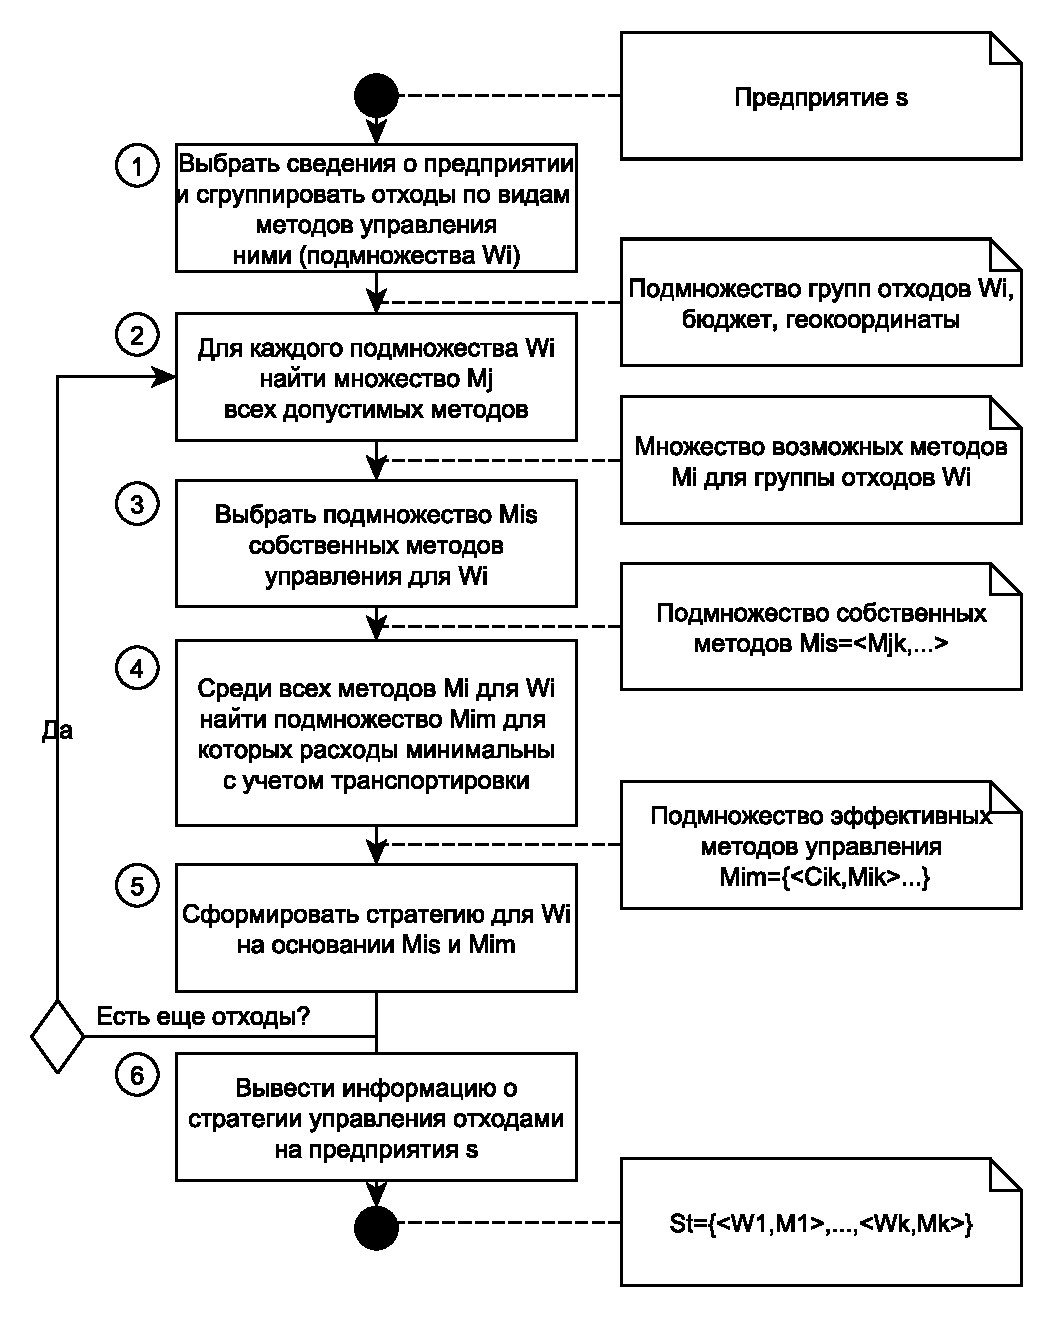
\includegraphics[scale=0.6]{algorithm}
\caption{Алгоритм генерации эффективной стратегии управления отходами на предприятии (верхний уровень)}
\label{fig:algorithm}
\end{figure}

В \textbf{четвертой главе} для автоматизации процесса поиска эффективной стратегии управления отходами на основе разработанных моделей и алгоритмов предложена архитектура интеллектуальной системы поддержки принятия решений (см. рисунок~\ref{fig:architecture}), включающая уровни интерфейса, логический уровень и уровень данных.

Цифрами на схеме обозначены: 1~---~клиент-серверное взаимодействие по протоколу HTTP (запрос-ответ); 2~---~ запрос на авторизацию пользователя в системе и доступа к ресурсам; 3~---~веб-маршруты до ресурсов системы; 4-7~---~обработка HTTP запросов на соответствующих контроллерах ресурсов; 8-11~---~взаимодействие с моделями ресурсов в БД и базе знаний; 12~---~взаимодействие с программной платформой Stardog через ее API для осуществления логического вывода на онтологиях и поиска знаний с использованием семантических запросов; 13~---~взаимодействие с базой данных MongoDB с помощью программной прослойки mongoose.

\begin{figure}[H]
\centering
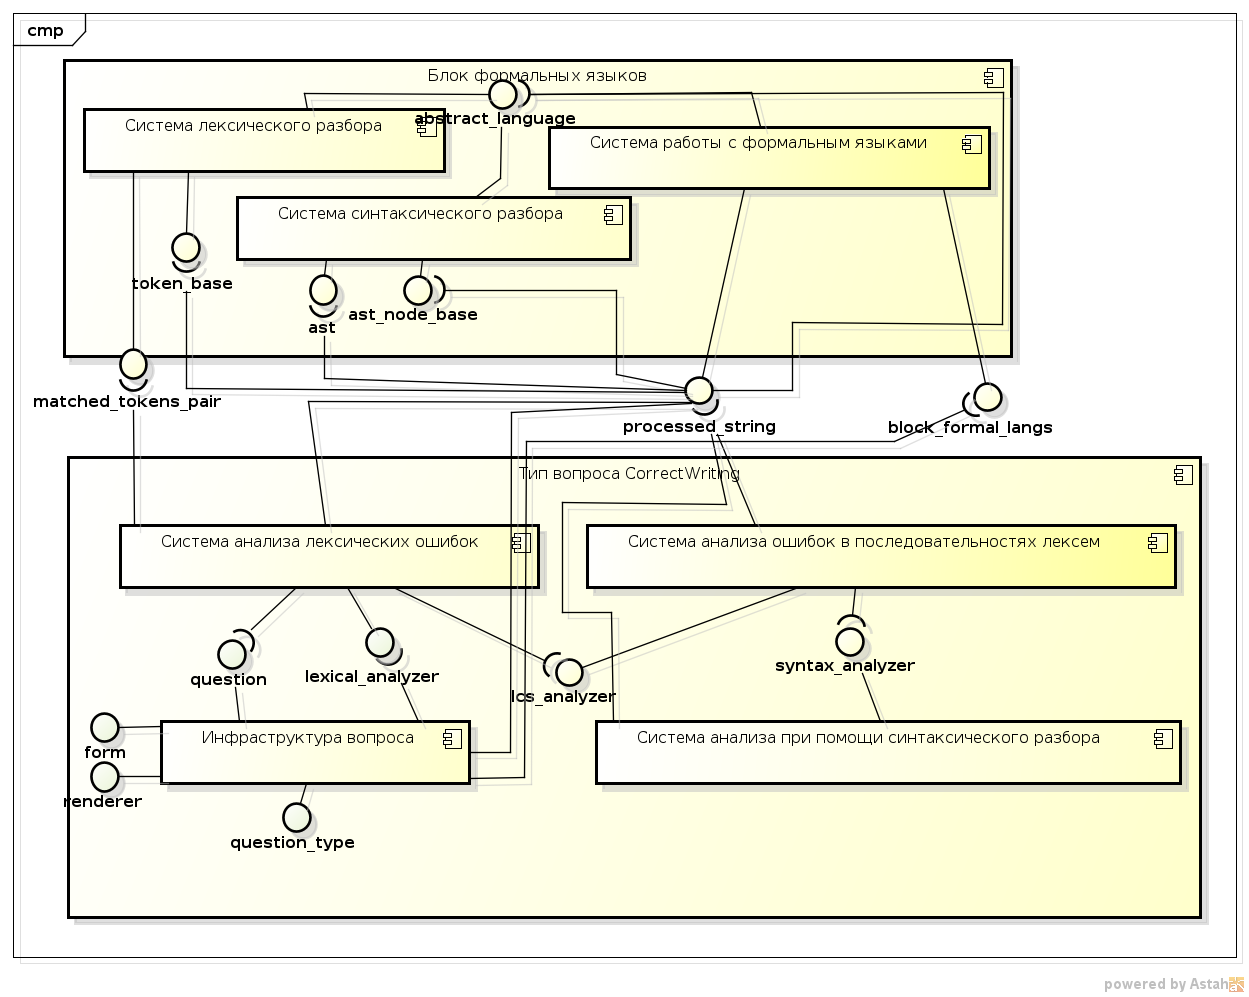
\includegraphics[scale=0.7]{component}
\caption{Архитектура системы поддержки принятия решений по управлению отходами}
\label{fig:architecture}
\end{figure}

Система поддержки принятия решений обладает клиент-серверной архитектурой и реализована на языке JavaScript. Для хранения онтологических знаний и проведения логического вывода на онтологиях используются программная платформа Stardog. Сгенерированная системой стратегия управления отходами отображается пользователю в браузере в виде структурированного списка в соответствии с предприятием, его отходами и доступными способами управления (см. рисунок~\ref{fig:screen_strategy_1} и~\ref{fig:screen_strategy_3}). 

%Пользователи системы подразделяются на администраторов и зарегистрированных пользователей.

%Зарегистрированный пользователь имеет возможность:
%\begin{itemize}
%\item просматривать каталоги отходов и методов управления отходами;
%\item создавать профиль предприятия, его отходы и способы управления;
%\item просматривать найденную стратегию управления отходами.
%\end{itemize}

%Администратор обладает всеми доступными правами и в дополнение к правам пользователя может:
%\begin{itemize}
%\item поддерживать базу знаний на основе онтологии;
%\item редактировать знания о предметной области управления отходами;
%\item добавлять пользователей в систему и редактировать их права.
%\end{itemize}

\begin{figure}[H]
\centering
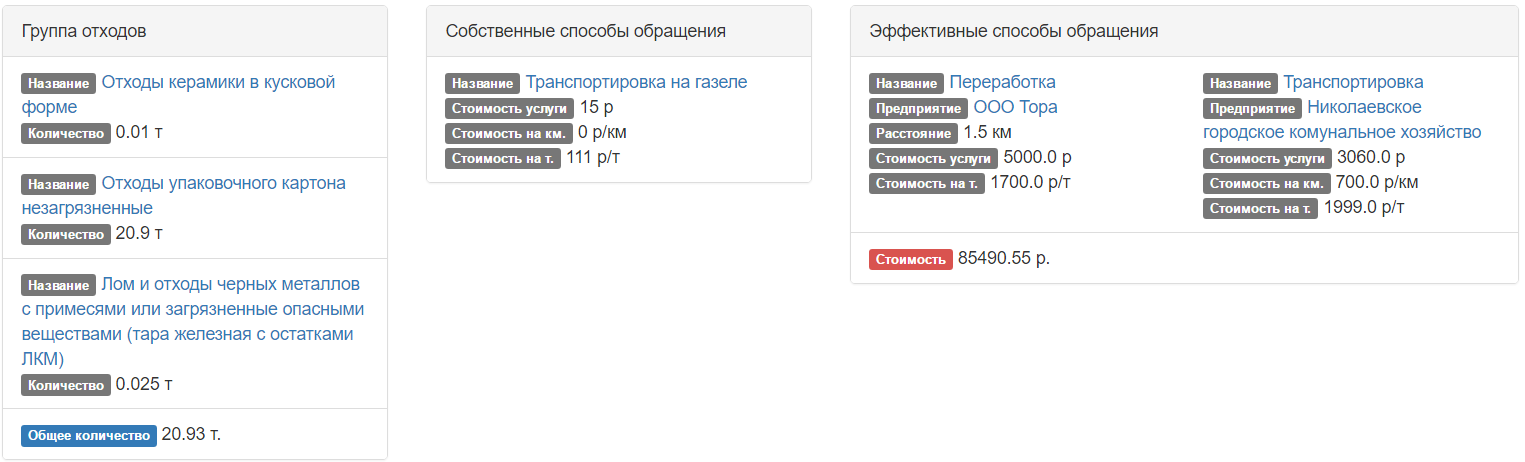
\includegraphics[scale=0.5]{screen_strategy_4}
\caption{Форма отображения сгенерированной стратегии управления отходами в системе (фрагмент 1)}
\label{fig:screen_strategy_1}
\end{figure}

\begin{figure}[H]
\centering
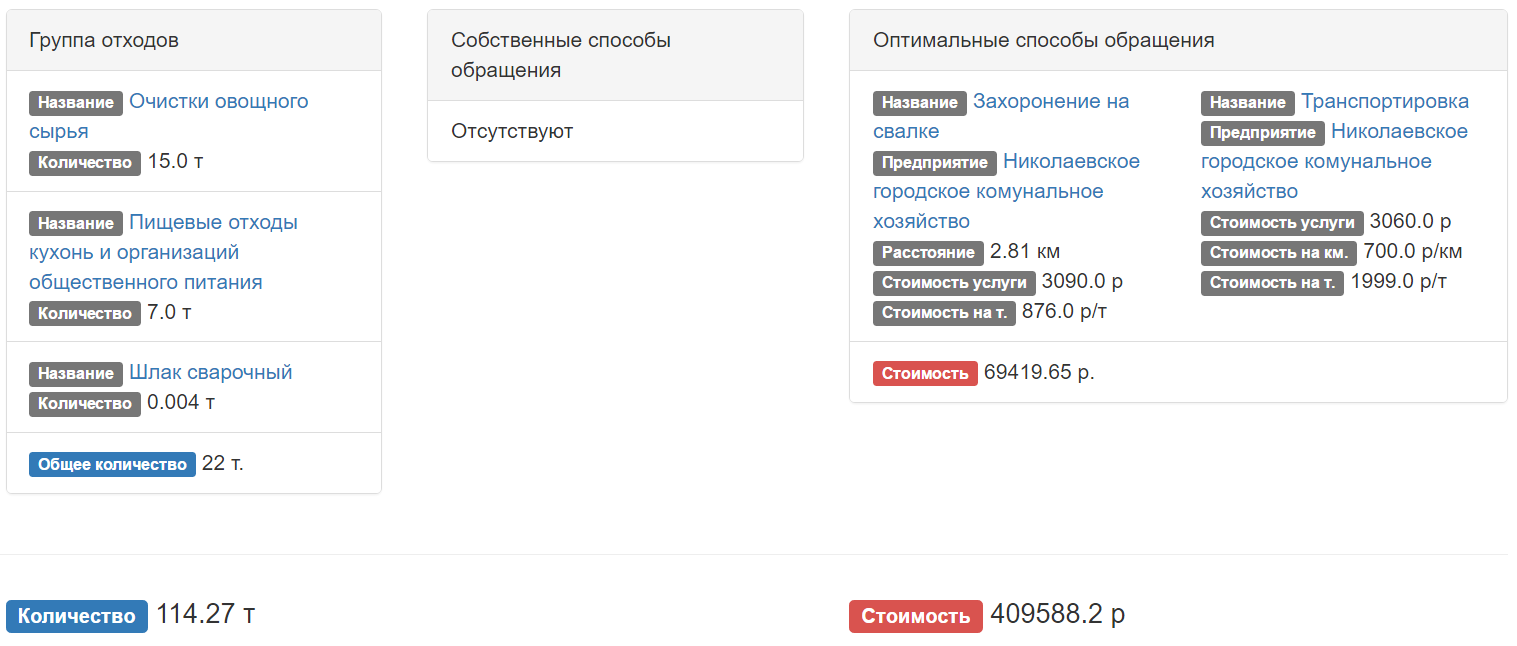
\includegraphics[scale=0.5]{screen_strategy_3}
\caption{Форма отображения сгенерированной стратегии управления отходами в системе (фрагмент 2)}
\label{fig:screen_strategy_3}
\end{figure}

Тестирование разработанного алгоритма генерации стратегии управления отходами проводилось на основании данных об учреждении ГБУЗ «Николаевское ЦРБ». Методика тестирования включала в себя следующие этапы: генерация эффективной стратегии управления отходами с помощью интеллектуальной системы поддержки принятия решений; сравнительный анализ результатов генерации стратегии с реальной политикой управления отходами на предприятии; оценка эффективности предложенной стратегии управления отходами.
Результаты тестирования показали, что выбранные системой способы управления отходами соответствуют способам управления, примененным в реальной политике обращения с отходами учреждения ГБУЗ «Николаевское ЦРБ»; для сгенерированной стратегии управления отходами полностью соблюдены законы и нормы РФ по обращению с отходами.
В целом результаты тестирования позволяют сделать вывод, что разработанные модели и алгоритмы адекватны поставленной задаче, а разработанная система может достаточно эффективно использоваться в качестве вспомогательного инструмента для поддержки принятия решений по управлению отходами на предприятии. 

В \textbf{заключении} диссертации приводятся основные научные и прикладные результаты, полученные автором в процессе выполнения работы.

\starchapter{ОСНОВНЫЕ РЕЗУЛЬТАТЫ И ВЫВОДЫ}

В процессе работы были решены следующие задачи и достигнуты следующие результаты:
\CommonResults

\clearpage

\starchapter{ОПУБЛИКОВАННЫЕ РАБОТЫ ПО ТЕМЕ ДИССЕРТАЦИИ}

\renewcommand{\theenumi}{\arabic{enumi}}
\renewcommand{\labelenumi}{\theenumi.}

\textbf{В изданиях, рекомендованных ВАК РФ}:
\CommonPublicationsVAK{}

\textbf{В прочих изданиях}:
\CommonPublicationsOther{}

\end{document}
